\section{Defining Safety Specifications for Synchronous Neural Networks}
\label{sec:definitions}

Chapter 3 introduced \acp{SNN} as time-predictable \acp{ANN} to address the timing verification of \acp{ANN} for \acp{CPS}.
The functional verification of \acp{ANN} has not yet been addressed.
This chapter tackles the problem of the functional verification of \acp{ANN} by proposing the combination of the previously defined \acp{SNN} and \acf{RE}~\cite{recps}.

\begin{figure}[h]
	\centering
	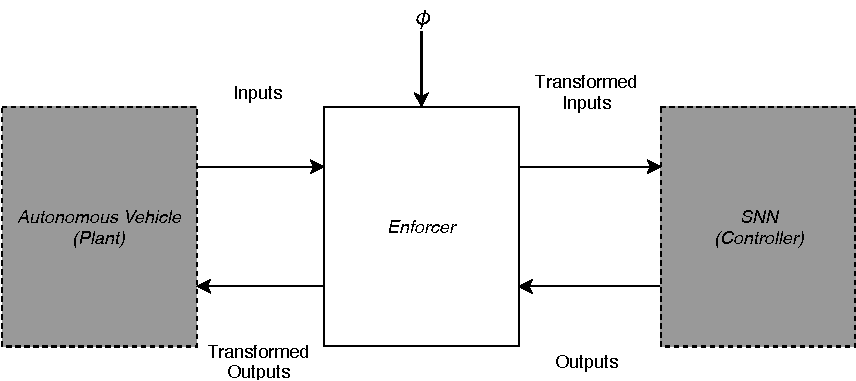
\includegraphics[width=0.8\linewidth]{Content/Fig/RE.pdf}
	\caption{Run-time enforcer between a \ac{SNN} and the \acf{AV}, to monitor the I/O events of the \ac{SNN}. \label{fig:re}}
\end{figure} 

We propose the use of bi-directional run-time enforcers~\cite{recps} to enforce the I/O events of \acp{SNN} at run-time.
These run-time enforcers are introduced in more detail in Chapter 2.
However, with the complex I/O of \acp{SNN}, an enforcer that edits only binary events is not sufficient.
Additionally, the edit functions introduced by \cite{recps} are not sufficient with more complex \ac{DTA}.
Consider Figure~\ref{fig:re}: we wish to enforce the inputs and outputs events of the \ac{SNN}, defined by some timed safety policy $\varphi$.
However, the outputs from the \ac{SNN} are 32-bit integer values, but the previously defined \acp{DTA} can only express binary signals.
Thus, we cannot use a \ac{DTA} to to specify the safety policies for this \acp{SNN}, nor can we enforce valued guards and transitions.
Instead, we propose the use of \acfp{VDTA}~\cite{rv-snn} to enforce valued I/O events of \acp{SNN}.

\subsection{\acf{VDTA}: Defining Safety Policies for \ac{CPS}}

We consider our industrial \ac{CPS} systems to have finite ordered sets of valued input channels ${I} = \{{i_1}, {i_2}, \ldots {i_n}\}$ and valued output channels ${O} = \{{o_1}, {o_2}, \ldots {o_n}\}$.
A VDTA can be seen as an automaton with a finite set of locations, a finite set of discrete clocks used to represent time evolution, and external input (resp. output channels) called ``external variables'' which are used for representing system data.
They also have internal variables which are used for internal computation, compared to the external variables which model the data carried by the actions from the monitored system (resp. environment). 
In a VDTA, a transition consists of an action carrying values of external variables, a guard on internal variables, external variables and clocks, and an assignment of internal variables, and reset of clocks.
%Thus, each input (resp. output channel) is considered as an external variable. 

Before we look into the formal definition of VDTA, let us consider an example.

\begin{example}
	The \ac{VDTA} for the pedestrian safety policy, $\mathcal{V}_{ped}$, is used for this example, and refers to the sensors in Figure~\ref{fig:av}.
	This \ac{VDTA} specifies that driving towards a pedestrian in-front of the vehicle (sensor 2) and not braking is a violation, and approaching a pedestrian from a distance (sensor 5) and not starting to slow down is also violation.
	This policy has been described in more detail in the previous section.
	
	This is encoded as a \ac{VDTA} with a set of locations $L = \{l_{drive}, l_{brake}, l_v\}$ and accepting locations $F = \{l_{drive}\}$, with the initial state being $l_{drive}$.
	The set of external variables $C = \{O_2, O_5, O_{2_v}, O_{5_v}, S\\, A, B_S, B_H\}$ are all 32-bit signed integers, where $O_2$, $O_5$, $O_{2_S}$, $O_{5_S}$ and $S$ are input channels and $A$, $B_S$ and $B_H$ are output channels.
	The set of actions $\Sigma = \{O_2, O_5, O_{2_S}, O_{5_S}, S, A, B_S, B_H\}$, and the set of internal variables $V = \{T_{lim}\}$, where $T_{lim}$ is a 32-bit signed integer.
	$X$, the finite set of discrete clocks, is limited to $t$ for this example: $X~=~\{t\}$.
	
	In this \ac{VDTA} there are two violation transitions, labelled \textcircled{a} and \textcircled{b} in Figure~\ref{fig:avpedrte}.
	\textcircled{a} occurs when the vehicle does anything else other than braking when there is a pedestrian in-front or not braking when there is no pedestrian ahead of the vehicle.
	\textcircled{b} can also occur when the vehicle has not braked enough within a certain period of time $T_{lim}$, or when the vehicle remains braking longer than is safe or necessary.
	This represents the vehicle taking further unsafe actions when already in an unsafe state.
\end{example}


Let us now consider in more detail the formal syntax and semantics of VDTAs.
%
For a variable (resp. channel) $v$, ${\cal D}_v$ denotes its domain,
and for a tuple of variables $V= (v_1, \ldots, v_n)$,
${\cal D}_V$ is the product domain ${\cal D}_{v_1} \times \cdots \times {\cal D}_{v_n}$.
%A predicate $P(V)$ on a tuple of variables $V$ is a logical formula whose semantics is a function ${\cal D}_V \rightarrow \{\true, \false\}$.
A valuation of the variables in $V$
is a mapping $\nu$ which maps every variable $v \in V$ to a value $\nu(v)$ in ${\cal D}_v$.
%
Let $X=\{x_1,\ldots, x_k\}$ be a finite set of integer variables representing discrete clocks.
%
A {\em valuation} for $x$ is an element of $\bbn$, that is a function from $x$ to $\bbn$.
The set of valuations for the set of clocks $X$ is denoted by $\chi$.
%
For $\chi\in\bbn^X$, $\chi+1$ (which captures the ticking of the digital clock) is the valuation assigning $\chi(x)+1$ to each clock variable $x$ of $X$.
Given a set of clock variables $X' \subseteq X$, $\chi[X' \leftarrow 0]$ is the valuation of clock variables $\chi$ where all the clock variables in $X'$ are assigned to $0$.

\begin{definition}[Syntax of {VDTA}s]
	\label{def:ptav}
	A {VDTA} is a tuple \\
	$\calA = \left(\Sigma, L, {l_0}, X, V, C, \Theta, F,  \Delta \right)$ where:
	\squishlist
	\item $\Sigma$ is a non-empty finite set of actions,
	and an action $a \in \Sigma$ has a signature $sig(a) = ( t_0, t_1, \ldots, t_k )$ which is a tuple of types of the external variables,
	\item $L$ is a finite non-empty set of locations, with $l_0 \in L$ the initial location, and $F \subseteq L$ the set of accepting locations;
	\item $X$ is a finite set of discrete clocks;
	\item $V$ is a tuple of typed internal variables; 
	\item $C$ is a tuple of external variables, where $C = I \cup O$, where $I$ is the set of input channels, and $O$ is the set of output channels; 
	\item $\Theta\subseteq {\cal D}_{V }$ is an initial condition which is a computable predicate over $V$;
	\item $\Delta$ is a finite set of transitions, and each transition $t \in \Delta$ is a tuple $( l, a, c, G, A, l' )$
	also written\\
	$l \xrightarrow{a(c), G(V,c), V':=A(V,c)} l'$
	such that,
	\squishlist
	\item[\textbullet] $l, l' \in L$ are respectively the origin and target locations of the transition;
	\item[\textbullet] $a \in \Sigma$ is the action, and $c=( c_1, \ldots c_k )$ is a tuple of external variables local to the transition;
	\item[\textbullet] $G = G^D \wedge G^X$ is the guard where
	\squishlist
	\item[-] $G^D \subseteq {\cal D}_V \times {\cal D}_{sig(a)}$
	is a computable predicate over internal variables and external variables  in $V \cup c$;
	\item[-] $G^X$ is a clock constraint over $X$ defined as a Boolean combinations of constraints of the form $x \sharp f(V \cup c)$, where $x \in X$ and $f(V \cup c)$ is a computable function, and $\sharp \in \{ <, \leq, =, \geq, > \}$;
	\squishend
	\item[\textbullet] $A$$=$$(A^D, A^X)$ is the assignment of the transition where
	\squishlist
	\item[-] $A^D :{\cal D}_V \times {\cal D}_{sig(a)} \rightarrow {\cal D}_V$ defines the evolution of internal variables.
	\item[-] $A^X \subseteq X$ is the set of clocks to be reset.
	\squishend
	\squishend
	\squishend
\end{definition}
%
A word is a sequence $\sigma = e_1\cdot e_2 \cdots e_n$ where $\forall i \in [1,n]: e_i = a_i(\eta_i)$ where $a_i \in \Sigma$ is an action and $\eta_i \in {\cal D}_V$ is a vector of values of a tuple of variables $V$. 

Policy \ac{VDTA} are required to be \textit{deterministic}, i.e. for any given state, the conjunction of any guards of any other outgoing transitions may not be satisfiable; and \textit{complete}, i.e. for any given state at any given time and any given event, at least one transition guard is satisfied.

\subsection{Semantics for \ac{VDTA}}

Let $\calA = \left(\Sigma, L, {l_0}, X, V, C, \Theta, F,  \Delta \right)$  be a VDTA.
The semantics of $\calA$ is a timed transition system,
where a state consists of a location, and valuations of internal variables $V$ and clocks $X$, and actions associated with values of external variables in $C$.

\begin{definition}[Semantics of {VDTA}s]
	\label{def:vdta:semantics}
	The semantics of $\calA$ is a timed transition system $\sem{\calA}=( Q, q_0, Q_F, \Gamma, \to )$, defined as follows:
	\squishlist
	\item $Q = L \times {\cal D}_V \times \bbn^X$, is the set of states of the form $q= ( l,\nu ,\chi )$ where
	$l \in L$ is a location,
	$\nu \in {\cal D}_V$ is a valuation of internal variables,
	$\chi$ is a valuation of clocks;
	\item $Q_0 = \{ ( l_0,\nu, \chi_{[X \leftarrow 0]} )  \mid \Theta(\nu)=\true \}$ is the set of initial states;
	\item $Q_F = F \times {\cal D}_V \times \bbn^X$ is the set of accepting states;
	\item $\Gamma = \{ a(\eta) \mid
	a \in \Sigma \wedge \eta \in {\cal D}_{sig(a)}  \}$ is the set of transition labels;
	\item $\to\subseteq Q\times \Gamma\times Q$  the transition relation
	is the smallest set of transitions of the form
	$( l,\nu,\chi \rangle \longrightarrow {a(\eta)} \langle l',\nu',\chi')$
	such that  $\exists ( l, a, c, G, A, l' ) \in \Delta$,
	with $G^X(\chi + 1) \wedge G^D(\nu, \eta) $ evaluating to {\true},
	$\nu'= A^D(\nu, \eta)$ and $\chi'=(\chi+1)[A^X \leftarrow 0]$.
	\squishend
\end{definition}


%The set of timed words over $\Sigma$ where the actions carry parameter value and other data is denoted by $\tw(\Lambda)$.
A {\em run} $\rho$ of $\sem{\calA}$ from a state $q\in Q$ over a {\em trace} $w =  a_1(\eta_1)\cdot a_2(\eta_2)\cdots a_n(\eta_n)$ is a sequence of moves in $\sem{\calA}$:
$\rho = q \xrightarrow {a_1(\eta_1)} q_1
\cdots q_{n-1}\xrightarrow {a_n(\eta_n)} q_{n}$,
for some $n\in\bbn$.
The set of runs from the initial state $q_0\in Q$,  is denoted $\Run(\calA)$ and $\Run_{Q_F}(\calA)$ denotes the subset of those runs {\em accepted} by $\calA$, i.e.,  ending in an accepting state $q_n \in Q_F$.

%%%%%%%%%%%%%%%%%%%%%%%%%%%%%%%%%%%%%%%%%%%%%%%
%%%%%%%%%%%%%%%%%%%%%%%%%%%%%%%%%%%%%%%%%%%%%%%
\ignore{
\begin{example}[Run of a VDTA]
	Let us consider the VDTA discussed in Example\ref{eg:vdta} presented in Figure~\ref{fig:vsa-overcurrent}. 
	An example run of the VDTA depicted in Figure~\ref{fig:vsa-overcurrent} is elaborated here.
	Let the internal variable $i_{max}$ be initialized with 10000.
	A run of this VDTA starting from the initial state $(l_{safe}, i_{max}=10000, x = 0)$ for the word $\sigma = tk(4000, 5000,1)\cdot tk(8000, 5000,1)\cdot tk(7000, 5000,1)\cdot tk(8000, 5000,1)\cdot tk(8000, 5000,1)\cdot tk(8000, 5000,1)$ is given below:\\
	$
	(l_{safe}, i_{max}=10000, x = 0)
	\xrightarrow {tk(4000, 5000,1)} \\
	(l_{safe}, i_{max}=10000, x = 1)
	\xrightarrow {tk(8000, 5000,1)} \\
	(l_{unsafe}, i_{max}=10000, x = 0)
	\xrightarrow { tk(7000, 5000,1)} \\
	(l_{unsafe}, i_{max}=10000, x = 1)
	\xrightarrow { tk(8000, 5000,1)} \\
	(l_{unsafe}, i_{max}=10000, x = 2)
	\xrightarrow { tk(8000, 5000,1)} \\
	(l_{unsafe}, i_{max}=10000, x = 3)
	\xrightarrow { tk(8000, 5000,1)} \\
	(l_{vio}, i_{max}=10000, x = 4).
	$
	
	The run started in the initial state and ended in a non-accepting state. It is thus a non-accepting run and represents a violation scenario.
}


\begin{example}[Run of a VDTA]
	\label{ex:run}
	An example run of the VDTA presented in Figure~\ref{fig:avpedrte} is presented here.
	The functionality of this \ac{VDTA} is explained in the previous section, and the \ac{AV} sensor positions are shown in Figure~\ref{fig:av}.
	Assume that the time the vehicle has to be braking is $T_{lim} = 3$. 
	The starting state is $l_{drive}$, and the first I/O event is $(\{0, 0, 0, 0, 2\}, \{\langle 0, 0, 0 \rangle\})$.
	The inputs show that nothing is detected in-front of the vehicle it is cruising at a fast speed km/h ($S~=~2$) and the vehicle does not accelerate or brake.
	Thus, the automaton remains in state $l_{drive}$.
	Next tick, $(\{0, 1, 0, 1, 2\}, \{\langle 0, 1, 0 \rangle\})$ occurs, i.e. a pedestrian ($O_5~=~1$) is detected quite far ahead of the vehicle, moving across the road at a slow pace ($O_{5_S}~=~1$), and the vehicle is taking a soft braking action ($B_S~=~1$) from a fast speed ($S~=~2$).
	Since the outputs ${O} = \{\langle 0, 1, 0 \rangle\}$, which is a soft brake $B_S$, and sensor 5 picks up a pedestrian a pedestrian $O_5~=~1~=~P$ the system enters the unsafe state $l_{brake}$ and $t~:=~0$ is set.
	Then,  $(\{1, 0, 0, 0, 1\}, \{\langle 0, 0, 0 \rangle\})$ is received, i.e. the pedestrian has stopped moving in the road and is now close to the vehicle ($O_2~=~P$), however the vehicle is not taking any action, but rather cruising at a slow speed ($S~=~1$).
	Since no braking is detected ($B_H~=~0$), the violation transition $l_v$ is taken.
	As such, this run was \textit{non-accepting}.
\end{example}

\subsection{Enforcing Non-accepting I/O Events}
Enforcers are designed to prevent a system from generating an input/output trace that is non-accepting, such as Example~\ref{ex:run}.
\cite{recps} proposed \ac{DTA} semantics with two possible methodologies for editing non-accepting I/O events.
These are \textit{random} and \textit{minimum} edits; a random edit chooses a random, accepting event from a list of accepting I/O events and minimum edit chooses the closest accepting event to the current non-accepting event.
However, neither of these edits always useful for problems in real scenarios.
Take Example~\ref{ex:run}, when the transition $l_{brake} \rightarrow l_v$ is taken because the vehicle does not slow down when approaching a pedestrian, $O_2$ can be edited to be nothing ($O_2~=~2$) so that $l_v$ is not entered, however this will not remove the danger that initially posed this transition since there really is a pedestrian in front of the vehicle.
However, if the action in output ${O}$ was changed, e.g. the cruising action ($\{\langle 0, 0, 0 \rangle\}$) in the example that caused the non-accepting trace was changed to a hard braking action ($\{\langle 0, 0, 1 \rangle\}$), then the transition back to $l_{brake}$ would have been taken \textit{and} the pedestrian in the road would have been safe.

In general, then, the designer of any given policy should also select their preferred edit actions out of the list of possible safe edits for each violation transition, thus ensuring practical runtime enforcement.

\begin{example}[Selected Edit Actions for a VDTA]
	In Figure~\ref{fig:avpedrte}, there are many different actions in $\Sigma$ that, when taken in a specific location $L$ result in a violation transition.
	In this example, a situation where the current location is $l_{drive}$ and the action is $\Sigma = \{1, 0, 1, 0, 1, 1, 0, 0\}$, i.e. there is a pedestrian directly in front ($O_2~=~1$) of the vehicle moving slowly, while the vehicle is moving directly forward slowly ($S~=~1$) and accelerating ($A~=~1$).
	Thus, the violation transition \textcircled{a} occurs.
	\squishlist
	\item Transition \textcircled{a}: $A := 0$, $B_S := 0$ and $B_H := 1$
	\squishend
	The recovery for this violation transition is to suppress the accelerate signal ($A~=~0$), and set the hard brake signal to present ($B_H~=~1$).
	This instead changes the transition to $l_{drive} \rightarrow l_{brake}$, which is a safe transition that slows the vehicle down before it hits the pedestrian.
\end{example}














